%!TEX TS-program = xelatex
%!TEX encoding = UTF-8 Unicode
\documentclass[11pt,a4paper]{article}

%\usepackage[left=70pt,top=50pt,bottom=70pt,right=40pt]{geometry}
\usepackage{amsmath}
\usepackage{amsfonts}
\usepackage{amssymb}
\usepackage{fixltx2e}
\usepackage{cmap}
\usepackage{enumerate}
\usepackage{ifthen}
\usepackage{listings}
\usepackage{url}
\usepackage[T1]{fontenc}
%\usepackage{fontspec}
%\usepackage{xunicode}
%\usepackage{xltxtra}
%\setmainfont[Mapping=tex-text,Ligatures={Common,Rare,Discretionary}]{Linux Libertine O}
\usepackage{pdflscape}
\usepackage{alltt}
\usepackage{algpseudocode}
\usepackage{wrapfig}
\usepackage{graphicx}

\ifthenelse{\isundefined{\hypersetup}}{
    \usepackage[colorlinks=true,linkcolor=blue,urlcolor=blue]{hyperref}
    \urlstyle{same}
}{}

\hypersetup{
    pdftitle={Intelligent Agents - EX1 - Yoan Blanc, Tiziano Signo}
}
\title{\phantomsection%
    A Reactive Agent for the Pickup and Delivery Problem
}
\author{
    Yoan Blanc \texttt{<yoan.blanc@epfl.ch>}, 213552\\
    Tiziano Signo \texttt{<tiziano.signo@epfl.ch>}, 226511
}
\date{\today}


\begin{document}
\maketitle

\noindent
\begin{quote}{\it

    At the beginning there are two tables:

    \begin{itemize}
        \item $p(i,j)$: The probability that in $\text{city}_i$ there is a task to be transported to $\text{city}_j$.
        \item $r(i,j)$: The reward for a task that is transported from $\text{city}_i$ to $\text{city}_j$.
    \end{itemize}

    \begin{enumerate}
        \item Define your state representation $S$, the possible actions $A$, the
            reward table $R(s,a) | s \in S, a \in A$ and the probability transition
            table $T(s,a,s') | s, s' in S, a \in A$.

        \item Implement the offline reinforcement learning algorithm for
            determining the actions to take in order to search and deliver
            tasks optimally. This algorithm should be executed before the
            vehicles start moving.

        \item Run simulations of one, two and three agents using your optimally
            learned strategy $V(S)$. Look at the performance graph of the agents.
            How does it change for different discount factor $\gamma$?

    \end{enumerate}
}\end{quote}

\newpage
\medskip
\textbf{State representation}

The space of states $S$ is defined by tuples of the current city ($curr$)
and the destination city ($dest$). We made this call because that what
is given to the agent as informations.

$$ \text{cities} = \{ \text{city}_1, \text{city}_2, \text{city}_3, \ldots, \text{city}_n \}$$

$$ S = \{ (curr, dest) \quad | \quad curr \in \text{cities}, dest \in
\text{cities} \cup \{ \emptyset \}, curr \neq dest \} $$

For example: $(city_i, city_j)$ represents the state where the agent is
in $city_i$ and there is a delivery to $city_j$ available to it. Likewise,
$(city_k, \emptyset)$ means that there are not tasks available to the agent
while it travels through $city_k$.

\medskip
\textbf{Action representation}

The space of actions $A$ is defined by accepting and delivering the proposed
task ($deliver$) or by deciding to move to another city.

$$ A = \{ action \quad | \quad action \in \text{cities} \cup \{\text{deliver}\} \} $$

\medskip
\textbf{Other definitions}

With the two spaces, we can now define the reward function $R(s,a)$ as well as
the state transition function $T(s,a,s')$ using $p(i,j)$ and $r(i,j)$. First,
define another function $q(i,j)$ which represents the cost to travel from
the $city_i$ to the $city_j$.

$$ q(i, j) = \text{cost per kilometer} * distance(city_i, city_j) $$

The reward function is defined as follow:

$$ R(s, a) = \left\{
    \begin{array}{l l}
        r(s.curr, s.dest) - q(s.curr, s.dest) & \text{if} \quad a \in \text{cities} \\
        q(s.curr, s.dest) & \text{if} \quad a = \text{deliver}
    \end{array} \right. $$

And the state transistion function:

% shall we only consider the neighbors city when not delivering packages?

$$ T(s, a, s') = \left\{
    \begin{array}{l l}
        p(s'.curr, s'.dest) & \text{if} \quad a = s'.curr \\
        p(s'.curr, s'.dest) & \text{if} \quad a = \text{deliver}, s.dest = s'.curr \\
        0 & \text{otherwise}
    \end{array} \right. $$

\medskip
\textbf{Algorithm}

We followed the algorithm from the slides. An extra variable $ Best$ is used to
store which $a$ was the $max$ one and not only the best value.

\begin{algorithmic}
    \Function{reinforcementLearning}{}
        \For{$s \in S$}
            \State $V(s) \gets 0$
        \EndFor
        \While{$error \leq \epsilon$}
            \For{$s \in S$}
                \For{$a \in A$}
                    $Q(s, a) \gets R(s, a) + \gamma \sum_{s' \in S} T(s,a,s') V(s')$
                \EndFor
            $V(s) \gets max_aQ(s, a)$
            \EndFor
        \EndWhile
    \EndFunction
\end{algorithmic}

\bigskip
\textbf{Implementation details}

We start defining specifically built classes for \texttt{State} and
\texttt{Action} in order to simplify the construction of reward and transition
matrices and the reinforcement learning algorithm computation.

The implementation of the agents is based on 2 functions: \texttt{setup} and
\texttt{act}, the first one handling the offline preprocessing, and the second
one used at runtime to decide what to do and where to go next from any city.

\begin{wrapfigure}{r}{.5\textwidth}
    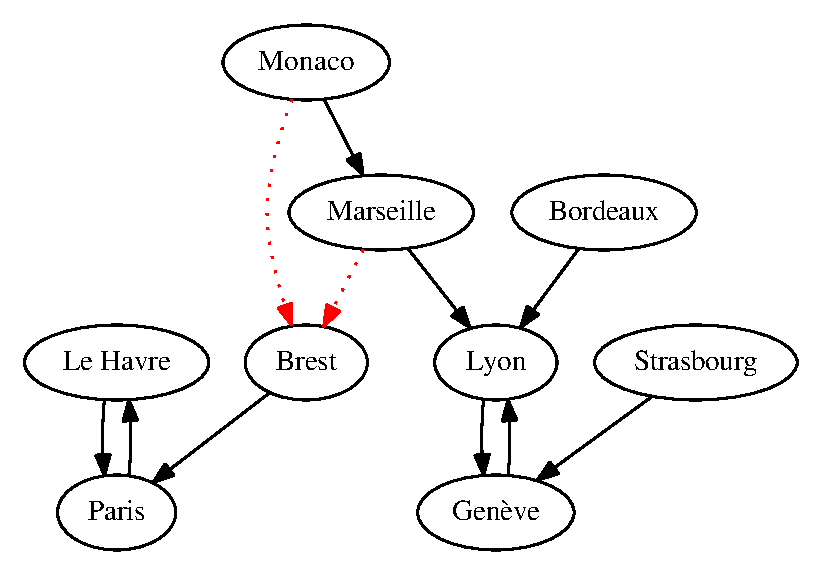
\includegraphics[width=.6\textwidth]{graph.eps}
    \caption{Default destination}{\textbf{solid lines} show where the agent will go if
        there are no tasks available\\\textbf{dotted lines} show the paths the agent
        will avoid by not reject the task.}
    \label{fig:graph}
\end{wrapfigure}

The function \texttt{setup} starts with the creation of our 4 basic structures
required for the reinforcemente learning algorithm:

\begin{enumerate}
    \item{\texttt{State} set (as an array of objects $s$)}
    \item{\texttt{Action} set (as an array of objects $a$)}
    \item{\texttt{Reward} matrix (as a matrix $s \times a$)}
    \item{\texttt{Transition} matrix (as a matrix $s \times a \times s'$)}
\end{enumerate}

The reward and transition matrices ensure that nothing forbidden is ever done
by returning the worst possible reward and $0$ probability in such cases. Having
this, the reinforcement learning algorithm is free of performing any further
checks.

When everything is computed the simulation can be started and here the focus is
moved to the \texttt{act} function. The function grabs the \emph{best} action
to take knowing the current state.

As we can see in the figure ~\ref{fig:graph}, the agents default path will tend
to find the best reward loop (a couple of cities to loop into) if there is no
tasks. But as long as the cost to move around is low proportional to the reward
the agent can get, it will tend to accept the tasks. To produce this figure, we
had to increase the$ cost per km$ quite a bit to get the agent to refuse accepting
some tasks (the red and dotted lines) and prefering moving to a better city
instead (the black and solid lines).

\bigskip
\textbf{Agents comparison}

\begin{wrapfigure}{r}{.5\textwidth}
    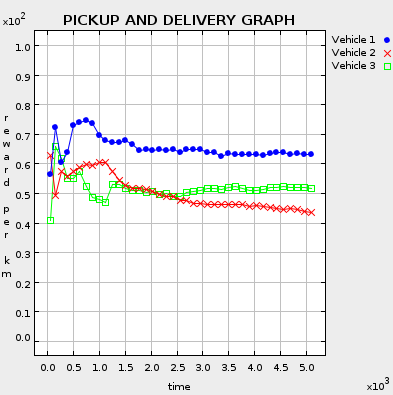
\includegraphics[width=.6\textwidth]{result.png}
    \caption{Result graph}{}
    \label{fig:result}
\end{wrapfigure}

In our simulation (see figure ~\ref{fig:result}), we show the map given in the
configuration and 3 agents operating on it. Each one of the agents follows a
different algorithm:

\begin{itemize}
    \item \textbf{Vehicle 1} reactive choice, take the best action according to the plan)
    \item \textbf{Vehicle 2} random choice, random choice to accept a task, move to
        random neighbor if not accepted)
    \item\textbf{Vehicle 3} greedy choice (always accept a task, move to random neighbor
        otherwise)
\end{itemize}

While the simulation runs it's possible to see the differences of rewards over
time and compare the efficiency of each agent. Our agent outperforms the other
ones, but not by a large margin. By always accepting tasks (the case when the
cost to move is low enough), the agent goes to cities to put it in not so good
situations.

\bigskip
\textbf{Conclusion}

Our agent seems to do its work even if the difference with the greedy one is
not impressive. Building a way to visualize the best actions space helped us to
fix our implementation and understand the observed behavior.

\end{document}
